\documentclass[10]{beamer}

%\renewcommand{\figurename}{}
%\usepackage[font={footnotesize,it}]{caption}
%
\usepackage{amssymb,latexsym,amssymb,amsmath,amsbsy,amsopn,amstext,upgreek}
\usepackage{color,multicol}
\usepackage{graphicx,wrapfig,fancybox,watermark,graphics}
\usepackage{picins}
%\usepackage{pgf}
%\usepackage{media9}
\usepackage{hyperref}
\hypersetup{
    pdfpagemode=FullScreen, % show in full screen?
}
\usepackage{pdfpages}

\usepackage{listings,bera}
\definecolor{keywords}{RGB}{255,0,90}
\definecolor{comments}{RGB}{60,179,113}
\lstset{language=C,
    keywordstyle=\color{keywords},
    commentstyle=\color{comments}\emph
}
\usepackage{algorithm}
\usepackage{algorithmic}
\renewcommand{\algorithmicrequire}{\textbf{Input:}}
\renewcommand{\algorithmicensure}{\textbf{Output:}}

% set fonts
%% \usepackage{fontspec}
%% %\setsansfont{Fontin Sans}
%% \setsansfont{Times}
%% \setbeamerfont{frametitle}{size=\LARGE,series=\bfseries}

%% \usepackage{xeCJK}
%% \usepackage{xltxtra}
%% %       beamer
%% % \usefonttheme{default} % sans serif
%% \usefonttheme{professionalfonts}
%% \usefonttheme{serif}

% reference entry
\usepackage{bibentry}
\usepackage[numbers]{natbib}

\usepackage[
    compress,
    %minimal,
    nonav,
    %red,
    %gold,
    blue,
    numbers,
    nologo,
    %polyu,
    comp,
    forty,
    %seventyfive,
]
{beamerthemeHongKong}

%
\usepackage{graphicx} % graphics
\usepackage{epsfig} % eps graphics
\usepackage{hyperref} % urls
\usepackage{booktabs, caption} % table styling

% suppress navigation bar
\beamertemplatenavigationsymbolsempty

%% \mode<presentation>
%% {
%%   \usetheme{bunsen}
%%   \setbeamercovered{transparent}
%%   \setbeamertemplate{items}[circle]
%% }

\mode<presentation>
{
%  \usetheme{Warsaw}
\usetheme{bunsen}       
  \setbeamercovered{transparent}
  \setbeamertemplate{items}[ball]
  \setbeamertemplate{theorems}[numbered]
  \setbeamertemplate{footline}[frame number]
}

% set fonts
\usepackage{fontspec}
%\setsansfont{Fontin Sans}
\setsansfont{Times}
\setbeamerfont{frametitle}{series=\bfseries} %size=\LARGE

% color definitions
\usepackage{color}
\definecolor{uipoppy}{RGB}{225, 64, 5}
\definecolor{uipaleblue}{RGB}{96,123,139}
\definecolor{uiblack}{RGB}{0, 0, 0}

% caption styling
\DeclareCaptionFont{uiblack}{\color{uiblack}}
\DeclareCaptionFont{uipoppy}{\color{uipoppy}}
\captionsetup{labelfont={uipoppy},textfont=uiblack}


%----------------------------------------
% see the macros.tex file for definitions
%\include{macros}
%---------------------------------

% adds reference to bottom right of corner of a slide
%% \usepackage[absolute,overlay]{textpos} % text references in slide corners
%% \newcommand\textref[1]{%
%%   \begin{textblock*}{\paperwidth}(0pt,0.99\textheight)
%%   \raggedleft \tiny{\emph{#1}}\hspace{.5em}
%%   \end{textblock*}}

% for drawing circles around numbers
% ex. \circled{1} Add some text here.
\usepackage{tikz}
\newcommand*\circled[1]{\tikz[baseline=(char.base)]{
            \node[shape=circle,draw,inner sep=2pt] (char) {#1};}}

%%--------
%\documentclass[11]{beamer}
\setbeamertemplate{navigation symbols}{}

\usepackage{beamerthemeshadow}
 

\usecolortheme[named=blue]{structure}

\mode<presentation>
{
  \usetheme{Warsaw}
  \setbeamercovered{transparent}
  \setbeamertemplate{items}[ball]
  \setbeamertemplate{theorems}[numbered]
  \setbeamertemplate{footline}[frame number]
}

% set fonts
\usepackage{fontspec}
%\setsansfont{Fontin Sans}
\setsansfont{Times}
\setbeamerfont{frametitle}{series=\bfseries} %size=\LARGE

 
%\usepackage{beamerthemeintridea}
 \usepackage{beamerthemesplit}
% \usetheme{Berkeley}
% \usetheme{Warsaw}
% \usecolortheme{dolphin}

%\usepackage{beamerthemesplit}
\usepackage{graphics}
\usepackage{graphicx}
\usepackage{hyperref}


\usepackage{amssymb,latexsym,amssymb,amsmath,amsbsy,amsopn,amstext,upgreek}
\usepackage{color,multicol}
\usepackage{graphicx,wrapfig,fancybox,watermark,graphics}
%\usepackage{picins}
%\usepackage{pgf}
%\usepackage{media9}
\usepackage{hyperref}
%\usepackage{booktabs, caption} % table styling
%\hypersetup{
%    pdfpagemode=FullScreen, % show in full screen?
%}

\mode<presentation>
{
  \usetheme{Singapore}
  \setbeamercovered{transparent}
  \setbeamertemplate{items}[ball]
  \setbeamertemplate{theorems}[numbered]
  \setbeamertemplate{footline}[frame number]
}
%\usecolortheme[named=dolphine]{structure}

%% % suppress navigation bar
\beamertemplatenavigationsymbolsempty

%========================================


\newcommand{\figdir}[1]{figures/#1}
\newcommand{\subdir}{}

\newcommand{\figref}[1]{Figure (\ref{#1})}
%\newcommand{\eqref}[1]{Eqn. (\ref{#1})}
\newcommand{\reffig}[1]{Figure (\ref{#1})}
\newcommand{\refeq}[1]{Eqn. (\ref{#1})}
\newcommand{\refsec}[1]{Section \ref{#1}}
\newcommand{\healpix}{HEALpix~}
\newcommand{\nside}[1]{N_{\rm side}}


\title{Possible application of the second order Gaussian Kinematic Formula to CMB
    data analysis}
  

\author[CMStatistics 2018]{Yabebal Fantaye}
\institute[Cape Town]{
  { African Institute For Mathematical Sciences (AIMS) \\
    South Africa} \\ 
\inst{} \\
 In collaboration with: D. Marinucci, V. Cammarota, \& A. P. Todino}


\date{\today} 


\begin{document}





%-----------------------------------------------------------------------------80
  \frame
  {
    \titlepage
  }


%-------------------------------------------------------------------
%                          Section 1
%-------------------------------------------------------------------
%
% Set the background for the rest of the slides.
% Insert infoline
%% \setbeamertemplate{background}
%%  {\includegraphics[width=\paperwidth,height=\paperheight]{slide_bg}}
%% \setbeamertemplate{footline}[bunsentheme]


%-----------------------------------------------------------------------------80
   \section*{Outline}
% %-----------------------------------------------------------------------------80
  \frame
  {
    \frametitle{Outline}

    \tableofcontents
  }


%-----------------------------------------------------------------------------80
\section{Introduction}
%-----------------------------------------------------------------------------80

\frame{

  \frametitle{Spherical Gaussian Random Fields}

  \begin{itemize}
\item In this talk all the results are presented for random eigenfunctions of $S^2$

%where $\Delta _{\mathbb{S}^{2}}$ is the Laplace-Beltrami operator on $%
%\mathbb{S}^{2}$

\begin{eqnarray*}
  \Delta _{\mathbb{S}^{2}}f_{\ell }+\lambda _{\ell }f_{\ell } &=&0,%
                                                                  \mbox{ }\mbox{ }\mbox{ }f_{\ell }:\mathbb{S}^{2}\rightarrow \mathbb{R}, \\
  \mathbb{E}[f_{\ell }(x)] &=&0,\mbox{ and }\mathbb{E}[f_{\ell }(x)^{2}]=1%
                               \text{,} \\
  \mathbb{E}[f_{\ell }(x)f_{\ell }(y)] &=&P_{\ell }(\cos d(x,y)),
\end{eqnarray*}%
where $\lambda _{\ell }=\ell (\ell +1),\mbox{ }\ell =0,1,\dots $, $P_{\ell }$ are the Legendre polynomials and $d(x,y)$ is the spherical
geodesic distance between $x$ and $y.$ The random fields $\{f_{\ell }(x),x\in \mathbb{S}^{2}\}
$ are Gaussian and isotropic.

\item \emph{Motivation}: Full-sky (inpainted) maps of the CMB have been released by Planck
2018; and see also A Rassat et al. (2014).

  \end{itemize}

}


\frame {
\frametitle{Geometry of Gaussian Random Fields}

\begin{itemize}

%\item Let $M$ be a general Riemannian manifold. In particular, for CMB we can think of $M$ as a sphere $S^2$.
\item  The basic set of random geometrical objects are $\mathcal{R}$
  valued random field $f(x)$ defined on $S^2$ and its excursion sets
  $A$, subregions where the value of $f$ exceeds the threshold $u$.

  \begin{equation}
    A_u(f, M) = \{ x \in M : f(x) \geq u \} 
  \end{equation}

%\item our interest here is to study the geometry e.g. peaks, isocontour lengths, area of these objects 

\end{itemize}

\begin{figure}
\begin{center}
\includegraphics[width=0.33\textwidth,angle=0]{\figdir{map_sup_u-3_fwhm5deg.pdf}} 
%\includegraphics[width=0.33\textwidth,angle=0]{\figdir{map_sup_u-2_fwhm5deg.pdf}} 
%\includegraphics[width=0.33\textwidth,angle=0]{\figdir{map_sup_u-1_fwhm5deg.pdf}} \\ 
\includegraphics[width=0.33\textwidth,angle=0]{\figdir{map_sup_u0_fwhm5deg.pdf}} 
%\includegraphics[width=0.33\textwidth,angle=0]{\figdir{map_sup_u1_fwhm5deg.pdf}} 
\includegraphics[width=0.33\textwidth,angle=0]{\figdir{map_sup_u2_fwhm5deg.pdf}} 
%\includegraphics[width=0.33\textwidth,angle=0]{\figdirTwo{map_sup_u3_fwhm5deg.pdf}} 
\end{center}
\end{figure}

}

%   Morphological properties are the characteristics of the field which are
%   invariant under translations and rotations and which are additive
%   i.e the Minkowski Functionals -  Area, Perimeter Length and Euler Poincar\'e characteristics
% }
% Note that for a digital image, one can consider a pixel as a compact and convex set.

% %----------------------------------------------
\frame {

  \frametitle{Morphological Properties}

  For a continuous functional $T$ on $\mathcal{R}$ 
  \begin{itemize}
    
    \item \emph{Translation and rotation invariant}:
      \begin{equation}      
        T(gK)=T(K) \mbox{ }\mbox{ } \forall K \in \mathcal{K}^d,
        \mbox{ } g\in G_d \mbox{ } \text{(group of
          rigid motions)}
      \end{equation}
      
  \item \emph{Additiv}: for convex sets (pixels) $\mathcal{K}^d$ in $\mathcal{R}^d$

    \begin{equation}
      T(K_1 \cap K_2) + T(K_1 \cup
      K_2) = T(K_1) + T(K_2)
    \end{equation}
    
    $K_1,K_2\in \mathcal{K}^n$ with $K_1 \cap K_2 \in \mathcal{K}^d$
    
  \end{itemize}
  
}

\frame {
  \frametitle{Steiner formula}

  \begin{itemize}
  \item  For convex, $M$, the volume, Lebesgue measure $\mu$, of a tube, $Tube(M,\rho) = \{
    t\in \mathcal{R}^n : dist(M,x)\leq\rho \}$,  with radius $\rho$ bounding $M$ is a polynomial
  in $\rho$ with terms of order $n, n-1, n-dim(M)$:

  \begin{equation}
    \mu(Tube(M,\rho)) = \sum_{j=0}^{n=dim(M)}{\omega_j\mathcal{L}_{n-j}(M)\rho^j}
  \end{equation}

  where $\mathcal{L}_j$ are the Lipschitz-Killing Curvatures; and  $w_j$ is the volume of a unit ball in $\mathcal{R}^j$.


  \item The Lipschitz-Killing Curvatures are related to Minkowski
  Functionals as $$\mathcal{M}_j(A) = (j!\omega_j)\mathcal{L}_{n-j}$$

  \end{itemize}

  }
  
    
  \frame {
    
  \frametitle{Lipschitz-Killing Curvatures}

    \begin{equation}
      area(Tube(A,\rho)) =
      \pi\rho^2\mathcal{L}_0(A)+\rho\mathcal{L}_1(A)+\mathcal{L}_2(A)
    \end{equation}

    \begin{picture}(100,100)
      \put(100,20){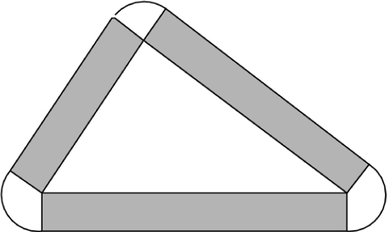
\includegraphics[width=0.33\textwidth,angle=0]{\figdir{misc/tube_triangle.png}}}
      \put(140,40){$A$}
    \end{picture}

    
    
    $\mathcal{L}_0$ - the Euler characteristics of A; \\
    $\mathcal{L}_1$ - half the boundary length of A; \\
    $\mathcal{L}_2$ - the area of A

}


\frame {

  \frametitle{Hadwiger Theorem (1959)}
  \begin{itemize}
    \item All properties of a d-dimensional convex set (or more generally, a finite union of convex
    sets e.g. pixels of a digital image) which satisfy the morphological properties are contained in d + 1 (LKC) values.\\

    \item For $\mathcal{K}^d$ the class of convex, compact sets in $\mathcal{R}^d$, a continuous map $T : \mathcal{K}^d \rightarrow \mathcal{R}$
    which satisfies the additive and rotation and translation invariance
    can be expressed as a linear combination of the LKCs
  \end{itemize}

  \begin{equation}
    T(K) = \sum_{i=0}^{d}\alpha_i \mathcal{L}_i(K) \hspace{1cm} \alpha_i\in \mathcal{R}
  \end{equation}


 % \begin{equation}
% T(gK)=T(K) \forall{K}\in \math{K}^d, g\in G_d  
% \end{equation}

% where $G_d$ is the group of rigid motions in $d$ dimensions (i.e.
% rotations and translations); and 

% \begin{equation}
% T(K_1 \intersection K_2) + T(K_1 \union
% K_2) = T(K_1) + T(K_2)
% \end{equation}
% for $K_1,K_2\in \mathcal{K}^n$
% with $K_1 \intersection K_2 \in \mathcal{K}^d$. Then
% $T$ can be expressed as a linear combination of the MFs

 
 }

  
  % ----------------------------------------------

% \frame {  
%   \frametitle{Lipschitz-Killing Curvatures (Minkowski Functionals) II}   
%     \begin{itemize}
%     \item $\mathcal{L}_{0}(A_{u}(f))$ is the genus or the
%       Euler-Poincar\`{e} characteristic (minima+maxima-saddles) of the
%       excursion regions. The third Minkowski functional. \\
%     \item $\mathcal{L}_{1}(A_{u}(f))$ is half the boundary length of
%       the excursion regions, e.g. the second Minkowski functional. \\
%     \item $\mathcal{L}_{2}(A_{u}(f))$ is the area of the excursion
%       regions, e.g.  the first Minkowski functional.
%     \end{itemize}       
%   }

%-----------------------------------------------------------------------------80
\section{Lipschitz-Kiling curvatures}

% -----------------------------------------------------------------------------80

\frame{
  \frametitle{Overview }

  \begin{itemize}
    \item A  lot  of  mathematical  effort to characterize  the  expected values of LKCs/MFs
      under Gaussianity culminated by the discovery of the powerful
      Gaussian  Kinematic  Formula (GKF)  by Adler \& Taylor.

      \item GKF leads to anaytical prediction of LKCs for a number of
        cases, e.g. harmonic \& needlet space.

      \item Several studies (on going) in recent years investigated
        characterizing the variance of LKCs/MFs in the high-frequency/high energy limit.
        starting from Wigman (2009) for the nodal length. A second
        order GKF like formula is emerging.

        %Cammarota, Marinucci \& Wigman for the excursion area,  Cammarota, Marinucci \& Wigman (2016) for the Euler-Poincar
        %characteristic, , Marinucci \& Wigman  for the critical values 
        
      \item The aim of this work is to present a unified overview of
        the literature, and especially to perform a detailed numerical investigation to verify the practical relevance of
        these results.
      \end{itemize}
  }
%-----------------------------------------
\frame {
  
  \frametitle{The Gaussian Kinematic Formula (GKF) }
  
  \begin{itemize}

  \item Developed by Adler \& Taylor, it is about expected
    values of Lipshitz-Killing curvatures for excursion regions.

  %% \[
  %% A_{u}(f):=\left\{ x\in S^{2}:f(x)\geq u\right\} \text{ .} 
  %% \]%
  
    \[
    \mathbb{E}\mathcal{L}_{i}(A_{u}(f,M))=\sum_{k=0}^{dim M - i}{i+k \brack k}
           {\mathcal{L}_{i+k}}(M)\mathcal{M}_{k}([u,\infty))
             \]
           
           {\small
             
             where given $\omega_i$ representing the volume of the $i^{th}$−dimensional unit ball
             \[
               {i+k \brack k} = {i+k \choose
                 k}\frac{\omega_{i+k}}{\omega_k\omega_i}                
               \]
           }
           
         \item $\mathcal{M}$ is given by
           {\small
             \[
             \mathcal{M}_j^{\gamma_k}([u,\infty))=(2\pi)^{-1/2}H_{j-1}(u)e^{-u^2/2}.
               \]
             }
             
             where $H_j$ is the Hermite polynomials: $H_0(u)=1$, $H_1(u)=u$, $H_2(u)=u^2-1$, $H_3(u)=u^3-3u$ 
  \end{itemize}
}

 

%-----------------------------------------------------------------------------80


\frame {

  \frametitle{The power of GKF }
  \begin{itemize}
  \item Splits the metric dependence of the field from that of
    excursion set behaviour.\\
    
  \item The $\mathcal{L}_{k}(M)$ part contains all the metric property. If
    the metric is scaled by $\lambda$, $\mathcal{L}_{k}(M)$ scales by
    $\lambda^k$. For spherical eigenfunctions, the scaling is
      $\lambda_{s}= \sqrt{\frac{s(s+1)}{2}}$ \\
    
  \item The $\mathcal{M}_{k}([u,\infty))$ part dependence only on the
    excursion threshold $u$. It absorbs all non-linear transformations:
    \begin{equation}
      H_{ns}(x):=H_{n}(f(x))=\frac{f^{n}(x)}{\sum_{l}b^{2}(\frac{%
          l}{B^{s}})\frac{2l+1}{4\pi }C_{l}}-1\text{ .} \text{where } n=2,3,..
      \end{equation}
  \end{itemize}  
  }

%--------------------------------------------------------

%-----------------

\frame{
\frametitle{Expected values of LKCs}

\begin{itemize}

\item The expected value of the first Lipschitz-Killing curvature (e.g. Euler-Poincar\`{e} characteristic)
\[
\mathbb{E}\mathcal{L}_{0}(A_{u}(f(x),S^{2}))=2\left\{ 1-\Phi
(u)\right\} + \lambda_{s}^2\frac{ue^{-u^{2}/2}}{\sqrt{(2\pi )^{3}}}4\pi \text{ ;} 
\]

\item The second Lipschitz-Killing curvature (e.g., half the boundary
length) 
\[
\mathbb{E}\mathcal{L}_{1}(A_{u}(f(x),S^{2}))=\pi \times  
\lambda_{s}e^{-u^{2}/2}\text{ ;} 
\]

\item The third Lipschitz-Killing curvature (e.g., the area of the
excursion region)
\[
\mathbb{E}\mathcal{L}_{2}(A_{u}(f(x),S^{2}))=4\pi \times \left\{
1-\Phi (u)\right\} \text{ .} 
\]%


\end{itemize}
}

\frame{
    \frametitle{Variances of LKC}
    The asymptotic behaviour of each of the three LKCs is dominated by a single, fully degenerate component,
    which can be written as:


\begin{eqnarray*}
\mathtt{Proj}[\mathcal{L}_{k}(A_{u}(f_{\ell };\mathbb{S}^{2}))|2]
&=&\frac{1}{2}\left[ 
\begin{array}{c}
2 \\
k%
\end{array}%
\right] \left\{ \frac{\lambda _{\ell }}{2}\right\}
^{(2-k)/2}H_{1}(u)H_{2-k}(u)\phi (u)\\
& &\frac{1}{(2\pi )^{(2-k)/2}} \int_{\mathbb{S}^{2}}H_{2}(f_{\ell }(x))dx+a_{k}(\ell ),
\end{eqnarray*}%

where
\begin{equation*}
a_{k}(\ell )=\left\{ 
\begin{array}{cc}
O_{p}(\ell ) & \text{for }k=0, \\ 
0 & \text{for }k=1,2%
\end{array}%
\right. \text{ .}
\end{equation*}%

}


  \frame {
    \frametitle{Simulation: Expected Values of LKCs}
  \begin{figure}
    \centering
    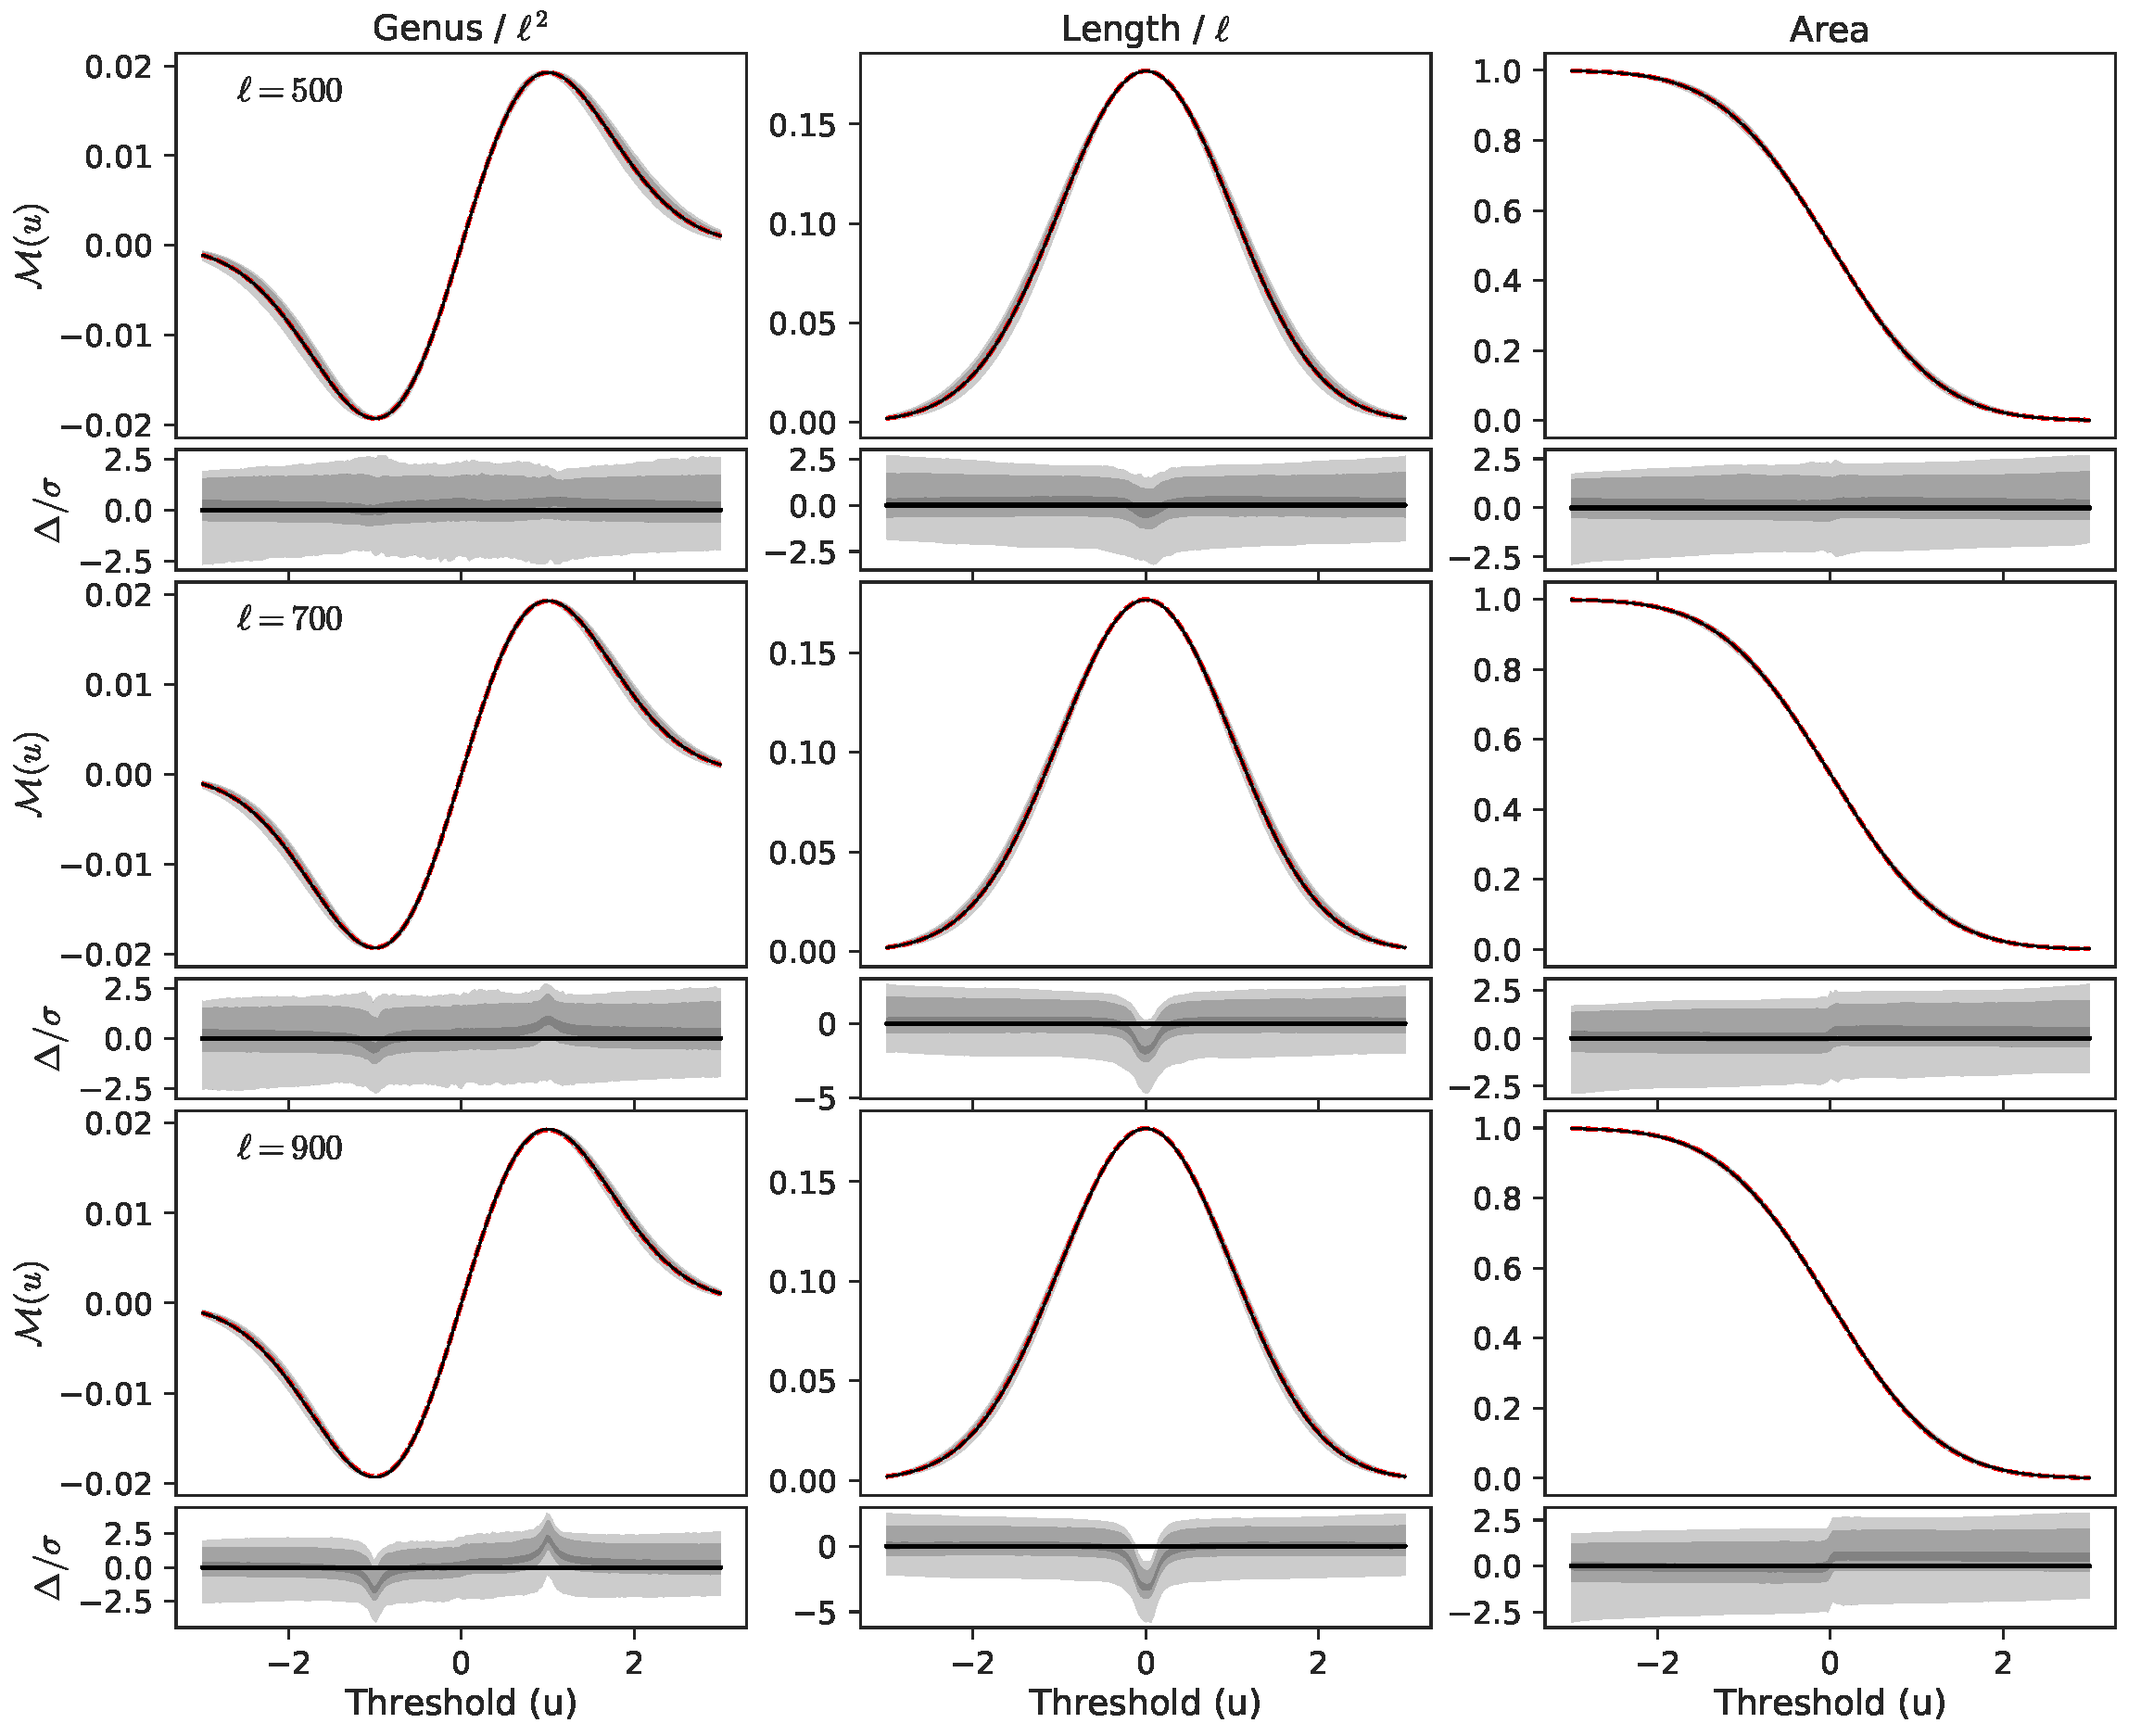
\includegraphics[width=0.8\textwidth]{\figdir{expVar/ap3_b200nj5_u201_3sig_ps0_sim_vs_try_mfs_ell.pdf}}
    \caption{ Analytical (red curve) vs Simulation (black and grey).} %1000 simulations.         
    \end{figure}    
  }

  \frame {
  \frametitle{Simulation: Variances of LKC}
  \begin{figure}
    \centering    
      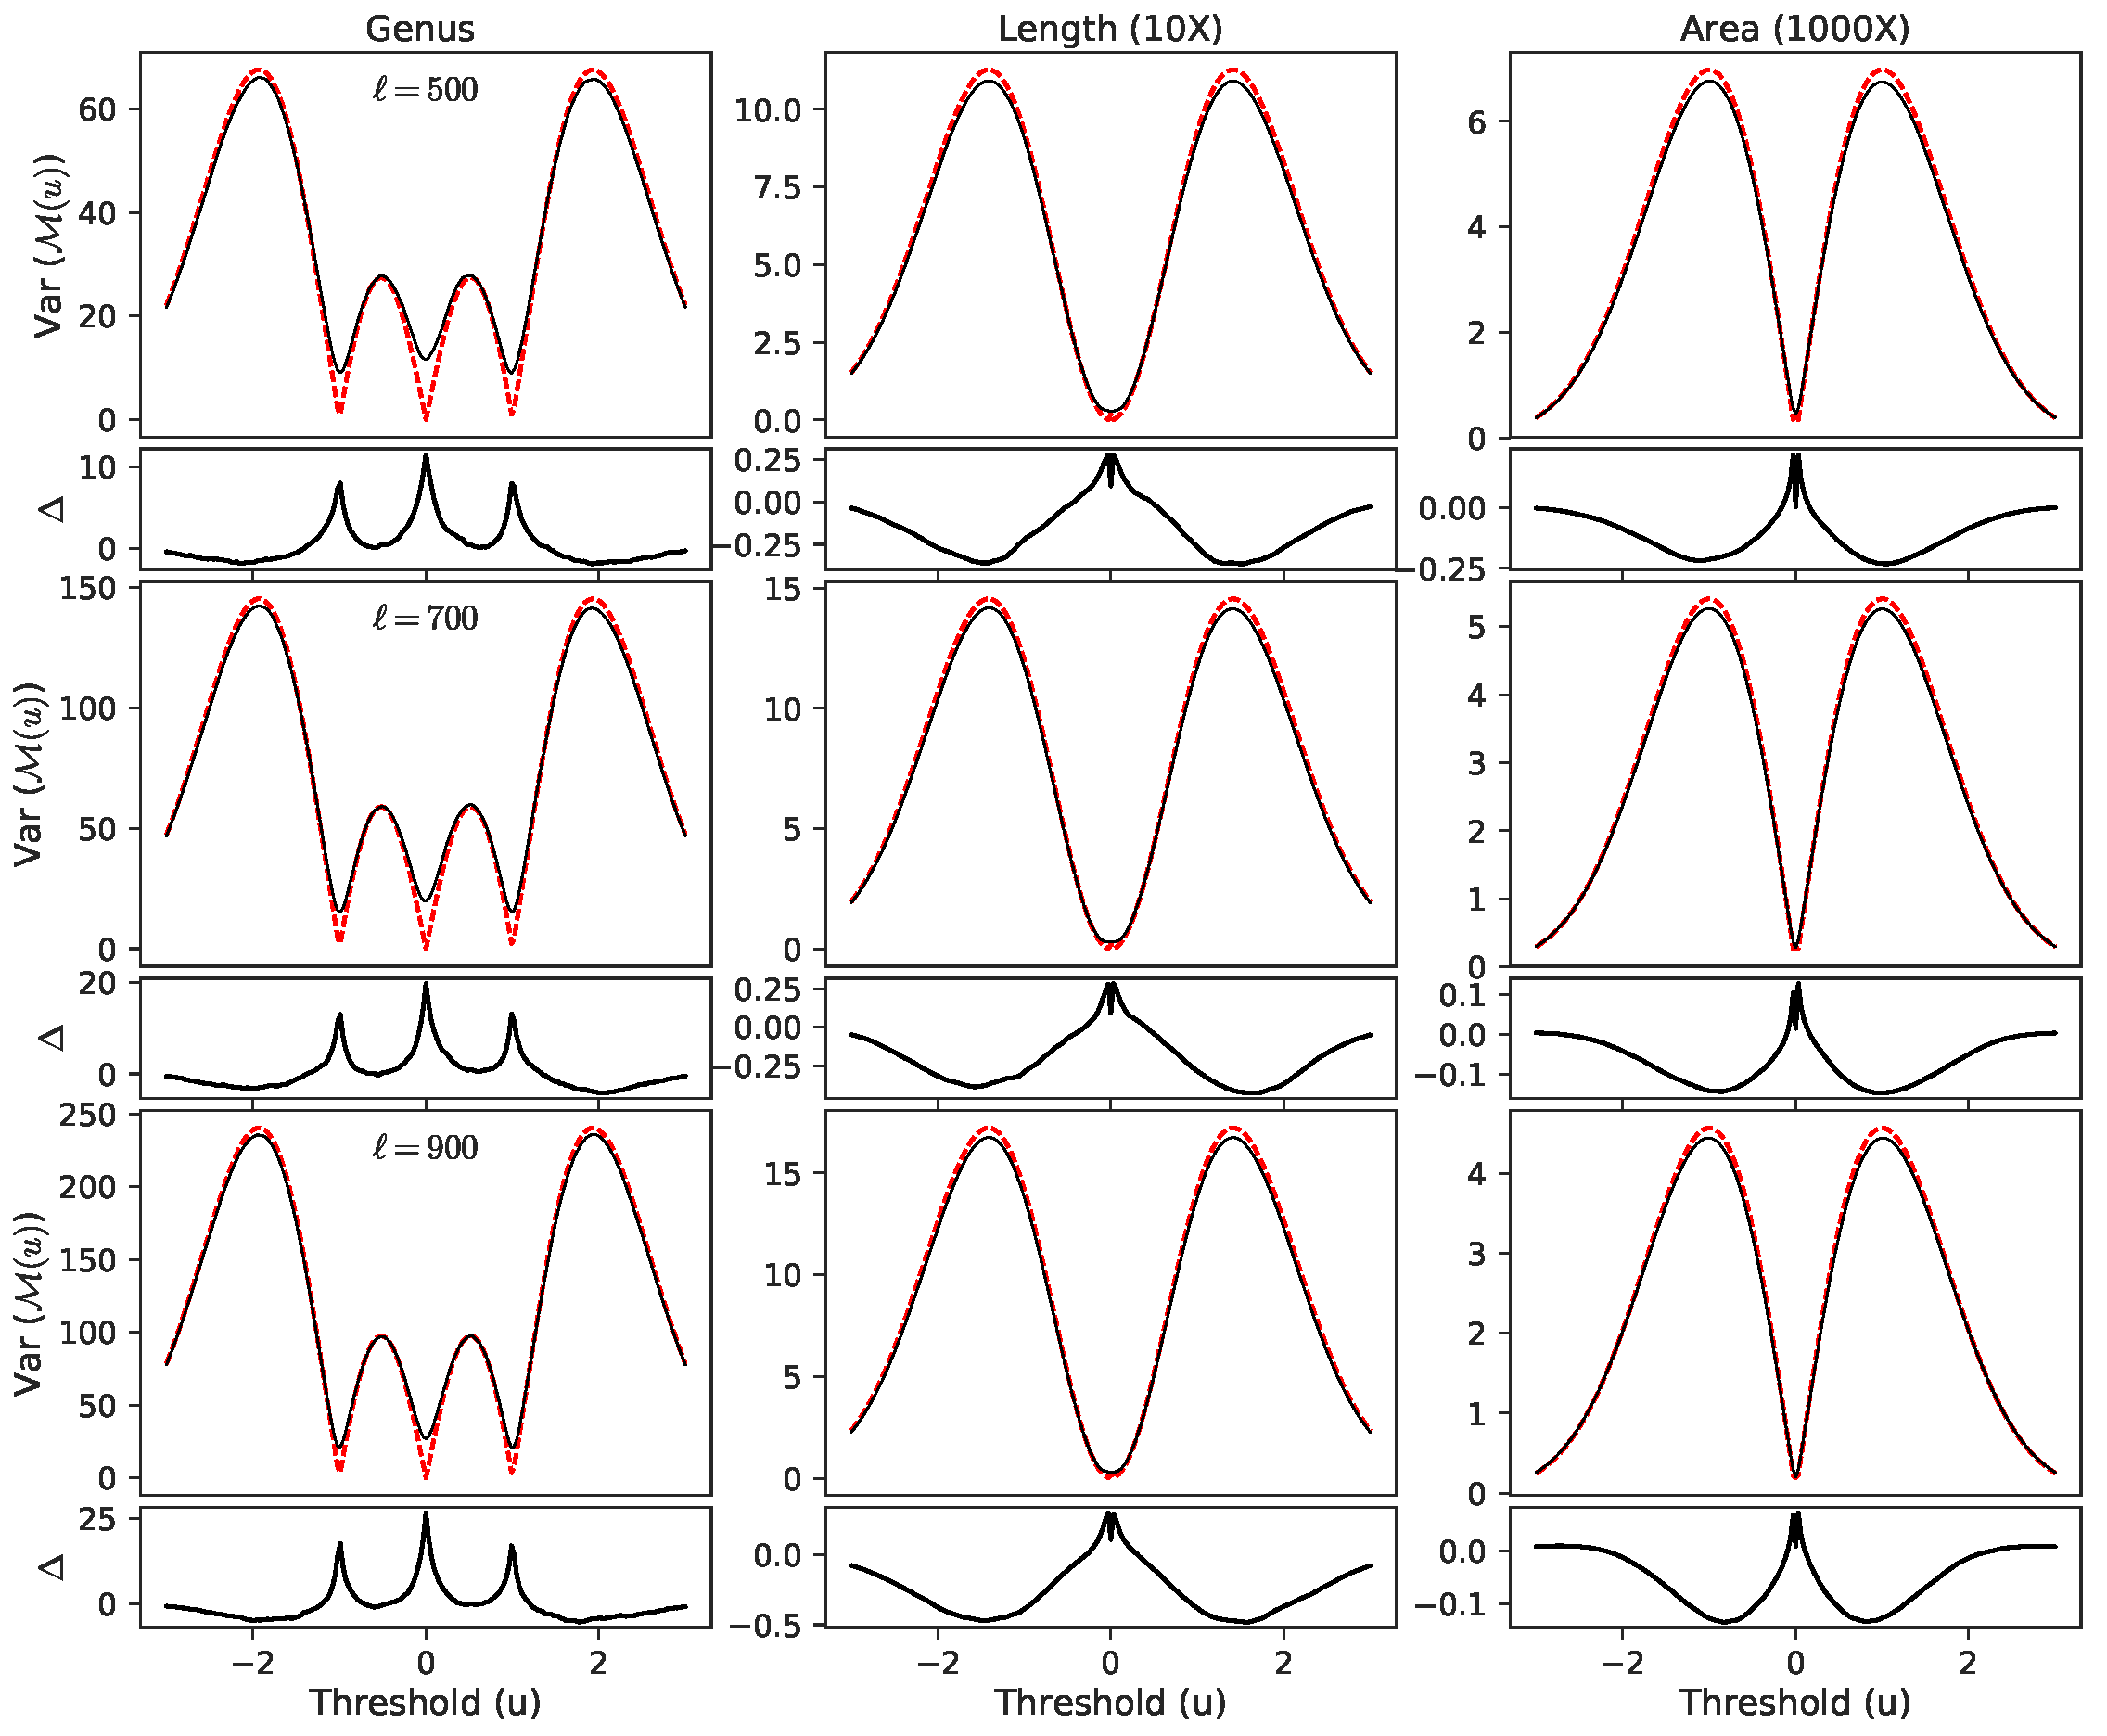
\includegraphics[width=0.8\textwidth,angle=0]{\figdir{expVar/ap3_b200nj5_u201_3sig_ps0_var_sim_vs_try_mfs_ell.pdf}}\\      
    \end{figure}
  }

%------------------------------------

\section{Critical points}
%------------------------------------

\frame{  
  \frametitle{Critical points, Extrema and Saddle }  
  \begin{equation*}
  \resizebox{.9 \textwidth}{!} {
$\mathcal{N}^{c}(f_\ell;u )=\mathcal{N}_{u}^{c}(f_{\ell })=\#\{x\in {\cal S}^2
:f_{\ell }(x)\geq u,\nabla f_{\ell }(x)=0\},$}
\end{equation*}

\begin{equation*}
  \resizebox{.9 \textwidth}{!} {
$  \mathcal{N}^{e}(f_\ell;u)=\mathcal{N}_{u}^{e}(f_{\ell })=\#\{x\in {\cal S}^2
:f_{\ell }(x)\geq u,\nabla f_{\ell }(x)=0,\text{det}(\nabla ^{2}f_{\ell
}(x))>0\},$}
\end{equation*}

\begin{equation*}
  \resizebox{.9 \textwidth}{!} {    
$\mathcal{N}^{s}(f_\ell;u)=\mathcal{N}_{u}^{s}(f_{\ell })=\#\{x\in {\cal S}^2
:f_{\ell }(x)\geq u,\nabla f_{\ell }(x)=0,\text{det}(\nabla ^{2}f_{\ell
}(x))<0\}.$}
\end{equation*}%
  }

  \frame{
  \frametitle{Expected values of Critical points}    
For every interval $u \in \mathcal{R}$ we have, as $\ell \rightarrow \infty$,
\begin{equation*}
\mathbb{E}[\mathcal{N}_{u}^{a}(f_{\ell })] =\frac{2}{\sqrt{3}} \ell(\ell+1) \int_{u}^{\infty}\pi _{1}^{a}(t)dt+O(1),
\end{equation*}
where $a=c,e,s$ and for the density
functions

\begin{align*}  
  \pi _{1}^{c}(t)&=\frac{\sqrt{3}}{\sqrt{8\pi
                   }}(2e^{-t^{2}}+t^{2}-1)e^{-\frac{                   
                   t^{2}}{2}}, \\
  \pi _{1}^{e}(t)&=\frac{\sqrt{3}}{\sqrt{2\pi
                   }}(e^{-t^{2}}+t^{2}-1)e^{-\frac{                   
                   t^{2}}{2}},\\
  \pi _{1}^{s}(t)&=\pi _{1}^{c}(t)-\pi
                   _{1}^{e}(t)=\frac{\sqrt{3}}{\sqrt{2\pi
                   }}e^{-\frac{3}{2}t^{2}}.\\
  \label{eqn:exp_crit}                                  
\end{align*}
}

\frame{
  \frametitle{Variances of Critical points}
  For every $u \in \mathcal{R}$ as $\ell \rightarrow \infty$
  
  \begin{equation*}
    {\text{Var}}(\mathcal{N}_{u}^{a}(f_{\ell }))=\ell^3 \left[
      \int_{u}^{\infty}p_{3}^{a}(t)dt\right] ^{2}+O(\ell^{2}\log^2 \ell),
  \end{equation*}
  where,
  
  \begin{eqnarray*}
    p_{3}^{c}(t)&=&\frac{1}{ \sqrt{8 \pi }}e^{-\frac{3}{2} t^{2}
                    }[2-6t^{2}-e^{t^{2}}(1-4t^{2}+t^{4})], \\
    p_{3}^{e}(t)&=&\frac{1}{ \sqrt{8 \pi }}e^{-\frac{3}{2} t^{2}
                    }[1-3t^{2}-e^{t^{2}}(1-4t^{2}+t^{4})],\\
    p_{3}^{s}(t)&=&\frac{1}{q \sqrt{8 \pi }}(1-3t^{2})e^{-\frac{3}{2}%
                    t^{2}}. \\
  \end{eqnarray*}  
  
  }
  
  \frame{
  \frametitle{Variances of Critical points}
  
  The leading constants for the variances can be written more
  explicitly as
  
  \begin{eqnarray*}
    \left[ \int_{u}^{\infty }p_3^c(t)dt \right]^{2} &=& \frac{1}{8 \pi} e^{- 3 u^2} u^2 (2+ e^{u^2}
                                                        (u^2-1))^2, \\
    \left[ \int_{u}^{\infty }p_3^e(t)dt \right]^{2} &=& \frac{1}{8 \pi}  e^{- 3
                                                        u^2} u^2 (1+ e^{u^2} (u^2-1))^2,\\
    \left[ \int_{u}^{\infty }p_3^s(t)dt \right]^{2} &=& \frac{1}{8 \pi}  e^{- 3 u^2} u^2.\\
  \end{eqnarray*}
  
  Note that the leading terms in the variances cancel in all cases at
  the threshold $u=-\infty$ as well as $u=0$; The former means the
  variance is smaller when we focus on the total number of critical
  points.

}
                                                   
\frame {
  \frametitle{Expected Values of critical points}
  \begin{figure}
        \centering
      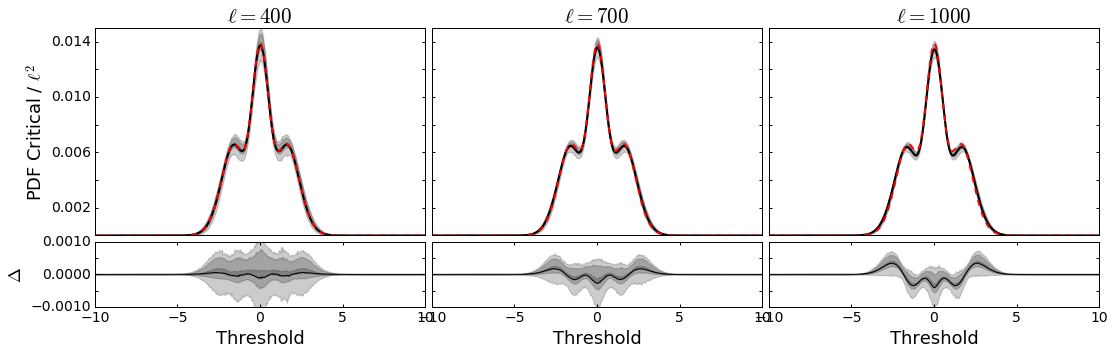
\includegraphics[width=0.7\textwidth,angle=0]{\figdir{expVar/criticals_multipole_nside2048_mean.png}}\\
      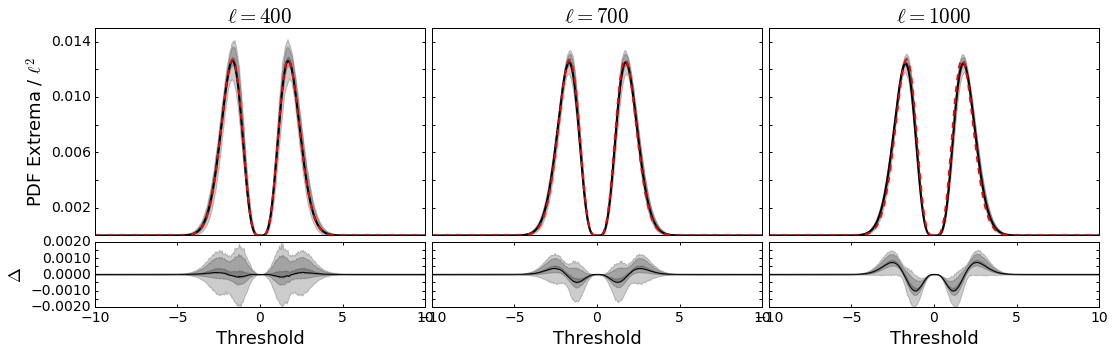
\includegraphics[width=0.7\textwidth,angle=0]{\figdir{expVar/extrema_multipole_nside2048_mean.png}}\\
      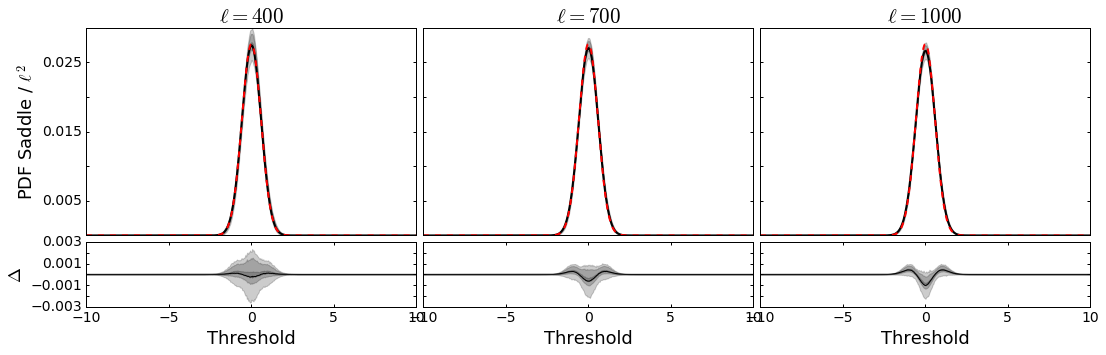
\includegraphics[width=0.7\textwidth,angle=0]{\figdir{expVar/saddles_multipole_nside2048_mean.png}}
      \caption{ Analytical (red curve) vs Simulation (black and
        grey).} %1000 simulations.            
    \end{figure}
  }


\frame {
  \frametitle{Variances of Critical points}
  \begin{figure}
    \centering    
      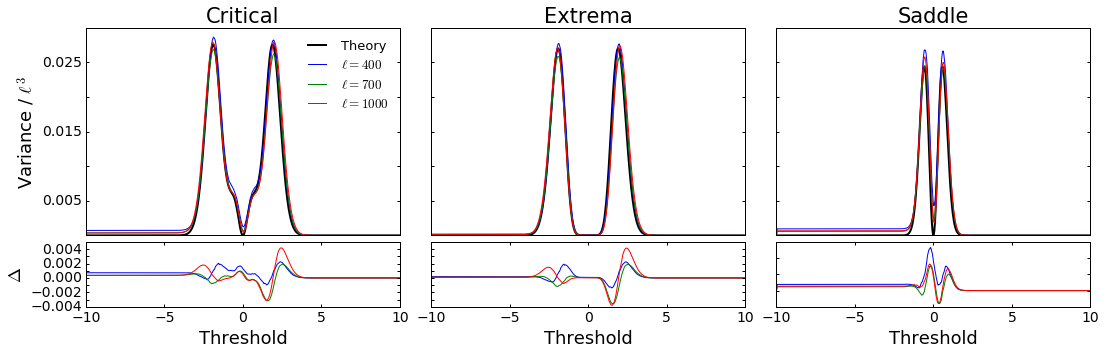
\includegraphics[width=1\textwidth,angle=0]{\figdir{expVar/var_crit_ext_sad_multipole_nside2048_mean.png}}
    \end{figure}
  }

\section{Correlations of LKC \& Critical points}  
\frame {
  \frametitle{Correlations}
  \begin{figure}
    \centering
    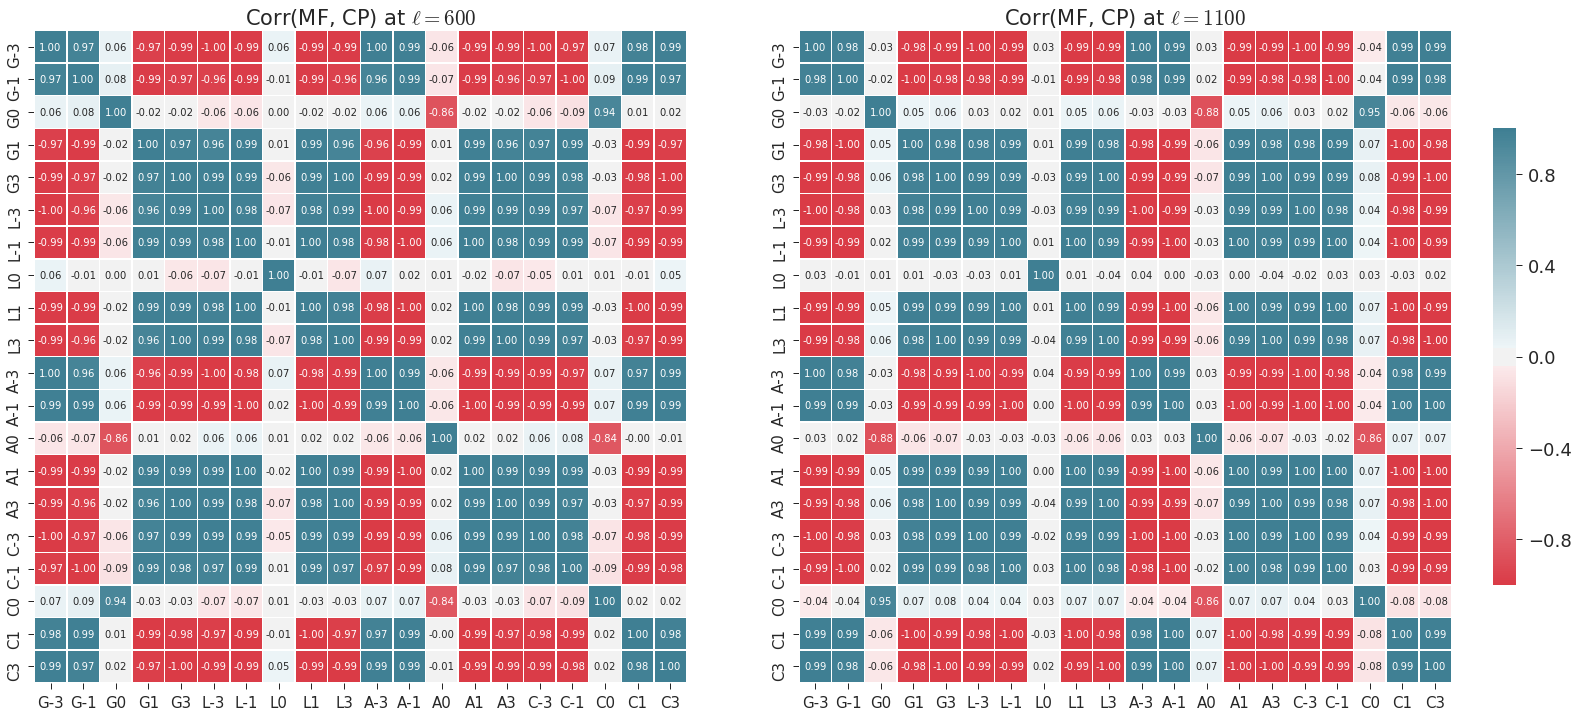
\includegraphics[width=1\textwidth,angle=0]{\figdir{expVar/ap3_b100nj10_u5_3sig_ps0_mfu_critu_corrcoef.png}}
  \end{figure}
  }


%--------------------------------------

\section{Summary}
%----------------------------------------

  
\frame {

\frametitle{Possible Applications}

What we have at the moment for Eigenfunctions of the sphere:
\begin{itemize}

\item Exact analytical predictions of the expected values of the LKCs
  (MFs) and accurate estimate on their variances.

\item Accurate analytical predictions of the expected values of
  critical points and their variances

\item Impurities, testing CMB inpainting algorithms for Gaussianity
  violation on MFs and peak statistics, etc.

\item Note that full-sky (inpainted) maps of the CMB have been released by Planck
2018; A Rassat et al. (2014) produced full sky CMB map.
  
\end{itemize}

}


\nocite{*}

%--------------------------------------------------
\begin{thebibliography}{99}
\bibitem{Adler e Taylor} Adler, R. J.; Taylor, J. E. (2007)
  \textit{Random fields and geometry}. Springer Monographs in
  Mathematics. Springer,
  New York. \\
  
\bibitem{CM}  Cammarota, V.; Marinucci, D. (2018) A
  Quantitative Central Limit Theorem for the Euler-Poincaré
  Characteristic of Random Spherical
  Eigenfunctions. \textit{Annals of Probabability }46, no. 6,
  3188–3228. \\

\bibitem{MV} Marinucci, D.; Vadlamani, S. (2016)
  High-Frequency Asymptotics for Lipschitz-Killing Curvatures
  of Excursion Sets on the Sphere. \textit{Ann. Appl. Probab.}
  26, no. 1, 462-506. \\
            
\bibitem{CMW} Cammarota, V.; Marinucci, D.; Wigman, I. (2016)
  Fluctuations of the Euler-Poincar\'e characteristic for random
  spherical harmonics,
  \textit{Proceedings of the American Mathematical Society}, 11,
  4759-4775. \\
  
  
\bibitem{CMW2016} Cammarota, V.; Marinucci, D.; Wigman,
  I. (2016) On the distribution of the critical values of random
  spherical harmonics, \textit{Journal of Geometric Analysis},
  4, 3252-3324.
	        
\end{thebibliography}




%%\item LKCs 
%% \item  the Lebesgue and Gaussian measure of the tube defines the Lipschitz-Killing Curvatures (LKCs) $\mathcal{L}_{k}(M)$ and Gaussian Minkowski Functionals (GMFS) $\mathcal{M}_{dim(M)-k}(M)$ respectively. 


%% \item  Let $\gamma=\gamma_k$ be a Gauss measure on $\mathcal{R}$ so that for $A \subset \mathcal{R}$
%% \[
%% \gamma_k(A) = (2\pi)^{-k/2}\int_A{e^{-|x|^2/2}dx}.
%% \]

%% \item now define a tube around $A$ such that
%%  \[
%%  \gamma_k(Tube(A,\rho)) = \gamma_k(A) + \sum_{j=1}^{\infty}{\frac{\rho^j}{j!}\mathcal{M}_j^{\gamma_k}(A)}
%% \]

%% \item $\mathcal{M}_j^{\gamma_k}(A)$ for $j \geq 1$ are called Gaussian MFs.

%%\item  For example for $[u,\infty)\subset R$

%%\item $\mathcal{M}_1$, $\mathcal{M}_2$, $\mathcal{M}_3$ are known as the \emph{area}, \emph{length} and \emph{genus} respectively.


\end{document}
